\chapter{Cadre du projet}
\minitoc
\clearpage
\section{Introduction}
\small{Vu que ce projet de fin d'études sera réalisé au sein d'une entreprise accueillante, il s'avère être indispensable d'avoir une idée sur cette dernière. Par la suite, nous allons mettre l'accent sur le sujet et les motivations derrière ce projet.}
\section{Présentation de l'organisme d'accueil}
Ce projet a été réalisé au sein du tout nouveau département IT de \textit{\textbf{Swiss Premium Negoce}} \cite{spn}.\\
\noindent Ce département se compose d'une équipe très innovante, très talentueuse qui est responsable des différentes applications et sites web de tous les différents services proposés par SPN.
\subsection{Présentation générale}
\vspace{1cm}
\begin{figure}[H]
    \centering
    
\includegraphics[width=0.25\textwidth]{spn_logo.png}
    \vspace{0.5cm}
    \caption{Logo Swiss Premium Negoce}
    \label{fig:spn_logo}
\end{figure}
\vspace{1cm}
\textit{\textbf{Swiss Premium Negoce SA}} (Société Anonyme) est une société de conciergerie basée à
Genève, Suisse. Créée en 2011 avec passion et enthousiasme, l'entreprise se spécialise en services de luxe.
En 2022, SPN a inauguré SPN Tunis avec son nouveau département IT, un département qui permettra d'atteindre plus d'audience à travers la digitalisation des différents services offerts par SPN.
\subsection{Activités}
SPN offre plusieurs services de luxe tel que:
\begin{itemize}
    \item Conciergerie
    \item Hospitalité de luxe
    \item Location de voitures
    \item Santé et services médicaux
    \item Camps d'été
    \item Éducation
    \item Jets privés
    \item Yachting
    \item Events
\end{itemize}
\section{Présentation du projet}
\subsection{Présentation générale}
L'application SPN-Cars est la solution trouvée par SPN pour offrir l'un de ses services les plus demandés plus facilement et convenablement grâce à l'utilisation de plusieurs nouvelles technologies qui permettront à l'entreprise de mieux performer et atteindre plus d'utilisateurs.\\
\noindent On doit alors définir ce projet, son objectif, ses concurrents, les problèmes qu'ils créent et comment l'application SPN-Cars pourra les corriger et offrir un service meilleur que les autres applications disponibles sur le marché.
\subsection{Problématique}
L'application SPN-Cars vise à devenir l'un des leaders dans les domaines de location de voiture en ligne, réservation de chauffeurs et des services taxis. Ce qui pose un grand défi : \textbf{Comment fournir aux utilisateurs de l'application ses services en tenant compte de la rapidité de l'application ainsi que la facilité des procédures ?}
\subsection{Étude de l'existant}
Il existe déjà plusieurs applications qui offrent des services similaires, chacune de ses applications présente des avantages et des inconvénients qu'on les explorera dans les chapitres suivants.
\phantomsection
\subsubsection{Sixt}
\vspace{1cm}
\begin{figure}[H]
    \centering
    
\includegraphics[width=0.25\textwidth]{sixt.png}
    \vspace{0.5cm}
    \caption{Logo Sixt}
    \label{fig:sixt_logo}
\end{figure}
\vspace{1cm}
Sixt \cite{sixt} est un fournisseur international de voitures de location, avec plus de 2000 véhicules dans 110 différents pays.\\
\noindent Sixt offre plusieurs services en rapport avec la location des voitures :
\begin{itemize}
    \item Location des voitures.
    \item Covoiturage.
    \item Service taxi.
    \item Location de voiture par abonnement mensuel.
\end{itemize}
\subsubsection{Blacklane}
\vspace{1cm}
\begin{figure}[H]
    \centering
    
\includegraphics[width=0.25\textwidth]{blacklane.jpg}
    \vspace{0.5cm}
    \caption{Logo Blacklane}
    \label{fig:blacklane_logo}
\end{figure}
\vspace{1cm}
Blacklane \cite{blacklane} est une entreprise allemande qui offre à ses clients la possibilité de réserver un chauffeur avec une voiture luxueuse et vivre une expérience VIP.\\
\noindent L'entreprise offre principalement trois services :
\begin{itemize}
    \item Trajets longue distance.
    \item Chauffeurs à la demande.
    \item Transfert aéroport.
\end{itemize}
\subsubsection{Uber}
\vspace{1cm}
\begin{figure}[H]
    \centering
    
\includegraphics[width=0.25\textwidth]{uber.jpg}
    \vspace{0.5cm}
    \caption{Logo Uber}
    \label{fig:uber_logo}
\end{figure}
\vspace{1cm}
Uber \cite{uber} est une entreprise de technologies américaine qui propose à ses clients une solution afin de trouver des chauffeurs pour les transporter vers leurs destination choisie grâce à son application mobile.\\
\noindent Uber a commencé en tant qu'une application qui joue le rôle d'intermédiaire entre ses utilisateurs et ses chauffeurs indépendants qui offrent leurs services.
\subsection{Critique de l'existant}
Même si les exemples mentionnés ci-dessus sont les leaders mondiaux dans le domaine des services de transport, ils sont tous différents. Surtout en termes de qualité de services, du marché visé.\\
\noindent Uber, par exemple, est à la recherche d'attirer un nombre maximal d'utilisateurs, c'est pourquoi l'application offre une sélection très variée de moyens de transport (voire fig. 5). Blacklane, par contre, vise une clientèle plus exclusive, une clientèle qui est prête à payer pour avoir un service de luxe. Ce qui est visible lors de la sélection de voitures à l'aide de l'application Blacklane comme le montre la figure ci-dessous (voir fig. 6)
\vspace{1cm}
\clearpage
\begin{multicols}{2}
    \begin{figure}[H]
        \centering
        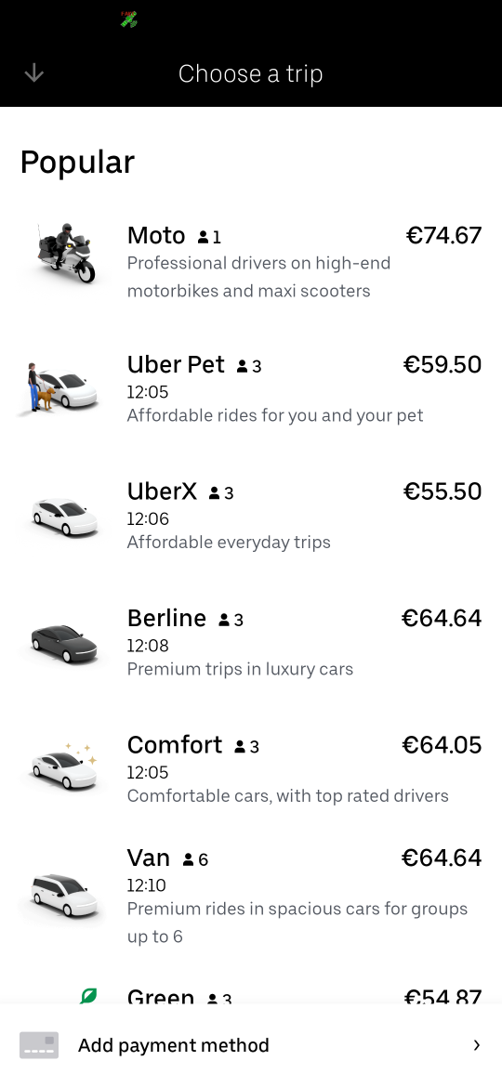
\includegraphics[height=0.5\textheight]{uber-car-selection.png}
        \vspace{1cm}
        \captionsetup{justification=centering}
        \caption{Sélection de voiture avec Uber}
        \label{fig:uber_selection}
    \end{figure}
    \begin{figure}[H]
        \centering
        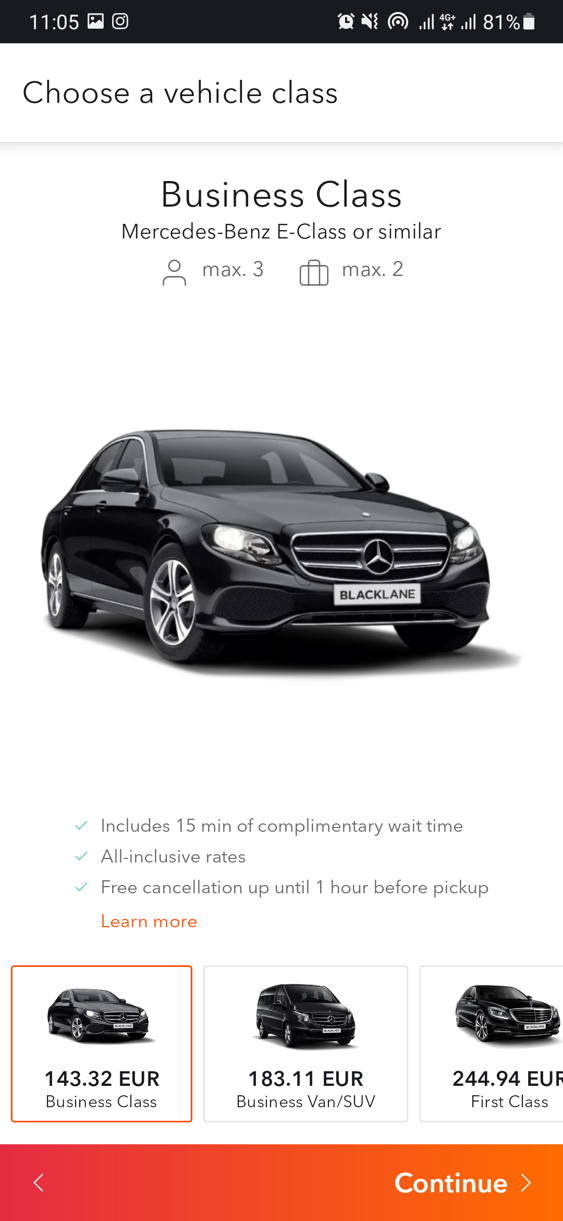
\includegraphics[height=0.5\textheight]{blacklane-car-selection.png}
        \vspace{1cm}
        \captionsetup{justification=centering}
        \caption{Sélection de voiture avec Blacklane}
        \label{fig:blacklane_selection}
    \end{figure}
\end{multicols}
\subsection{Solution Proposée}
% TODO : FInish this section
L'objectif de l'application SPN-Cars est de fournir à ses utilisateurs des expériences luxueuses en simples clics.\\
L'application doit être simple et permet aux utilisateurs d'avoir une expérience rapide et satisfaisante.
\begin{figure}[H]
    \centering
    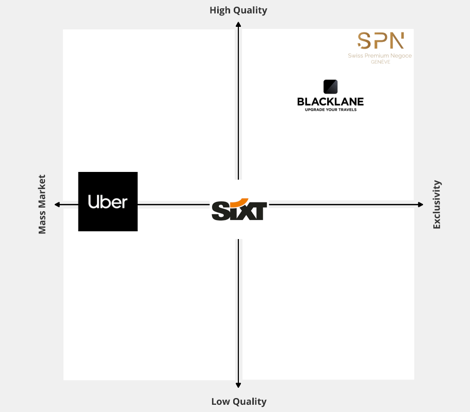
\includegraphics[height=0.5\textheight]{positionnement.png}
    \vspace{1cm}
    \caption{Positionnement de l'application SPN-Cars par rapport aux alternatives.}
    \label{fig:positionnement_marche}
\end{figure}
\section{Méthodologie de travail}
L'objectif est de pouvoir mener ce projet en respectant les délais et les budgets alloués. Pour atteindre cet objectif, il faut adopter une méthode de gestion de projet. Il existe de nombreuses méthodes à choisir dont on cite :
\begin{itemize}
    \item \textbf{Les méthodes traditionnelles: }Ces méthodes sont les plus utilisées en gestion de projet. Elles sont appelées également <<En cascade>> car chaque étape, car chaque étape doit être terminée pour passer à la suivante. En appliquant cette méthodologie, l'équipe projet suit le cahier de charges à la lettre et travaille sur la totalité du projet jusqu'à sa livraison. Il n'y a pas d'interaction avec le client qui recevra son projet une fois que celui-ci est terminé.
    \item \textbf{Les méthodes agiles :}Ces méthodes sont moins rigides que les méthodes traditionnelles, elles placent les besoins du client au centre des priorités du projet. Elles offrent une plus grande flexibilité et une meilleure visibilité dans la gestion du projet, ce qui permet à l'équipe d'être plus réactive aux attentes du client. Le projet sera découpé en mini-projets chacun nécessitant la validation du client pour passer au suivant.
\end{itemize}
\subsubsection{Comparaison des méthodes}
Chaque méthode présente des avantages et des inconvénients, il faut alors les comparer pour identifier la méthode appropriée pour ce projet.\\
\noindent Dans le tableau suivant on présente une comparaison des méthodes :\\
\begin{table}[H]
    \begin{center}
        \begin{tabularx}{0.8\textwidth} {
                | >{\centering\arraybackslash}X
                | >{\centering\arraybackslash}X
                | >{\centering\arraybackslash}X |}
            \hline
                              & Méthodes classiques                                                                    & Méthodes agiles                                                                                                                \\
            \hline
            Cahier de charges & Un cahier de charge complet doit être disponible.                                      & Se concentrent sur la phase de développement, le cahier de charges est souvent incomplet.                                      \\
            \hline
            Temps passé       & Le client n'est impliqué qu'au phases de conception et livraison de l'application.     & L'équipe de développement et le donneur d'ordre communiquent constamment pour échanger sur le projet et planifier les sprints. \\
            \hline
            Type de projet    & Ces méthodes sont préférées pour les projets complexes où rien n'est laissé au hazard. & Cette méthode convient aux projets incertains et innovants.                                                                    \\
            \hline
        \end{tabularx}
        \captionsetup{justification=centering}
        \caption{Comparaison des méthodologies de travail}
        \label{tab:meth_compare}
    \end{center}
\end{table}
\subsubsection{Méthode retenue}
Comme pour ce projet il existe un cahier de charges bien défini, et un temps de développement très strict, le choix d'une méthode classique, en particulier la méthode en cascade, est imminent.

La méthode en cascade est une méthode linéaire des différentes phases du projet nécessaires pour la création du livrable.\\
\noindent La méthode en cascade est composée de six étapes:
\begin{itemize}
    \item \textbf{Étape des exigences} : C'est la première étape où on définit les exigences et les besoins.
    \item \textbf{Étape de l'analyse} : Faire une analyse plus approfondie des solutions qui répondent aux besoins et écarter celles qui ne correspondent pas aux exigences.
    \item \textbf{Étape de conception} : Dans cette étape on va définir d'une façon détaillée les différents besoins.
    \item \textbf{La mise en œuvre} : Une fois tout est défini et accepté par tous les participants, on commence la partie de mise en œuvre où on développe les différentes fonctionnalités.
    \item \textbf{La validation} : Cette étape consiste à tester les fonctionnalités développées dans l'étape précédente une par une et corriger les problèmes rencontrés.
    \item \textbf{La mise en service} : À la fin de l'étape de validation le projet est mis en service.
\end{itemize}
\vspace{1cm}
\begin{figure}[H]
    \centering
    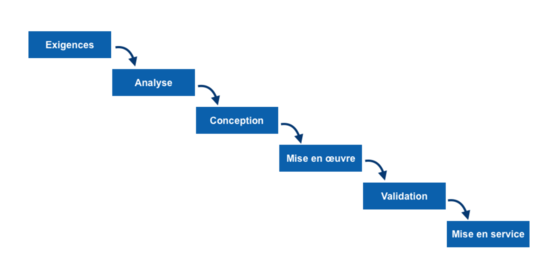
\includegraphics[width = \textwidth]{cas.png}
    \captionsetup{justification=centering}
    \caption{Méthode en cascade .}\cite{cascade}
    \label{fig:cascade}
\end{figure}

\section{Conclusion}
Dans ce chapitre, on a commencé par la présentation de l'entreprise accueillante et ses différentes activités. Puis on a présenté le projet offert et la problématique qu'il pose. Suite à la problématique, il fallait faire une étude de l'existant où on a pris l'exemple de différentes applications qui offrent un service similaire et déduisent leurs faiblesses. Une fois ces défauts dégagés, on a pu passer à la présentation de la solution proposée qui permettra de résoudre les points manquants des autres applications. Finalement on a présenté la méthodologie de travail suivie qui assurera la fluidité au niveau de la gestion de ce projet.\\
Suite à ce chapitre, on passera vers l'étape de conception où on définira les différents aspects du projet.